\section{Lecture 18}
``I again don't remember so I'll guess.''

\subsection{The Fourier Transform Revisited}
Recall
\begin{definition}
    Let $f: \mathbb{R}\to\mathbb{C}$. The, the Fourier Transform of $f$ is given by
    \begin{align}
        \hat{f}(\xi) = \dfrac{1}{\sqrt{2\pi}} \int_{-\infty}^\infty f(x) \cdot e^{-ix\xi} \dd{x}
    \end{align}
\end{definition}

\subsection{Some (more) Properties}
``In all of these examples, I forgot to divide by $1/\sqrt{2\pi}$, but it doesn't matter.''
\begin{enumerate}
    \item Linearity.
    \begin{align}
        \widehat{\left[f + g\right]} = \widehat{f} + \widehat{g}
    \end{align}
    \begin{proof}
        It's quite trivial to prove this using (18.1).
    \end{proof}
    \item Dilation. If $g(x) = f(ax)$, then
    \begin{align}
        \hat{g}(\xi) = \dfrac{1}{a} \hat{f}(\xi/a)
    \end{align}
    \begin{proof}
        Doing a substitution $y = ax$ and $\dd{y} = a\dd{x}$,
        \begin{align}
            \hat{g}(\xi) = \int f(ax) e^{-ix \xi} \dd{x} = \frac{1}{a}\int f(y) e^{-iy \frac{\xi}{a}} \dd{y}
        \end{align}
    \end{proof}
    \item Translation. If $g(x) = f(x+a)$, then $\hat{g}(\xi) = e^{ia\xi} \hat{f}(\xi)$, i.e. the Fourier transformation is multiplied by some trigonometric wave.
    \begin{proof}
        \begin{align}
            \hat{g}(\xi) = \int f(x+a) e^{-ix \xi} \dd{x}
        \end{align}
        Using $y = x + a$,
        \begin{align}
            \hat{g}(\xi) &= \int f(y) e^{-i(y-a) \xi} \dd{y}\\
            &= e^{ia\xi} \int f(y) e^{-iy \xi} \dd{y}
        \end{align}
        which equals
        \begin{align}
            \hat{g}(\xi) = e^{ia\xi} \hat{f}(\xi)
        \end{align}
    \end{proof}
    \item Modulation. If $g(x) = f(x) \cdot e^{iax}$, then
    \begin{align}
        \hat{g}(\xi) = \hat{f}(\xi - a)
    \end{align}
    \begin{proof}
        \begin{align}
            \hat{g}(\xi) &= \int f(x) \cdot e^{iax} \cdot e^{-ix\xi} \dd{x}\\
            &= \int f(x) \cdot e^{-ix(\xi-a)} \dd{x}\\
            &= \hat{f}(\xi - a)
        \end{align}        
    \end{proof}
\end{enumerate}

\subsection{Radio}
\subsubsection{AM (Amplitude Modulation) Radio}
Let $S(x)$ be some signal. AM radio broadcasts $S(x) \cdot e^{ixa}$, or the signal modulated by some trignometric wave. Some circuit then takes the Fourier transform of a signal, throws away all frequencies that don't matter, and then does an inverse Fourier transform. So, all other stations become damped.
\begin{align}
    \widehat{S(\xi) \cdot e^{i\xi a}} = \hat{S}(\xi + a)
\end{align}

\subsubsection{FM (Frequency Modulation) Radio}
Amplitude is held constant, but frequency changes.
\begin{figure}[H]
    \centering
    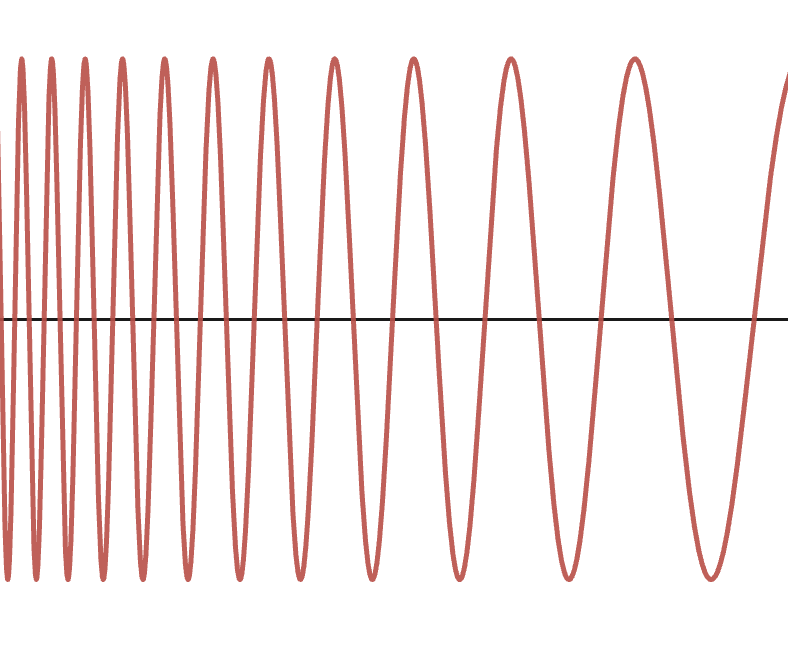
\includegraphics[width=0.45\linewidth]{image2.png}
    \caption{Frequency modulation}
\end{figure}

\subsection{Convolutions for Nonperiodic Functions}
\begin{definition}
    If $f, g \in V$, then their convolution is
    \begin{align}
        (f * g)(x) = \int_{-\infty}^\infty f(t) \cdot g(x-t) \dd{t}
    \end{align}
\end{definition}
\begin{enumerate}
    \setcounter{enumi}{4}
    \item Convolutions.
    \begin{align}
        \boxed{\widehat{f*g}(\xi) = \sqrt{2\pi} \cdot \hat{f}(\xi) \cdot \hat{g}(\xi)}
    \end{align}
    \begin{proof}
        \begin{align}
            \widehat{f*g}(\xi) &= \dfrac{1}{\sqrt{2\pi}} \int (f*g)(x) e^{-ix\xi} \dd{x}\\
            &= \dfrac{1}{\sqrt{2\pi}} \int \left[ \int f(t) \cdot g(x-t) \dd{t} \right] e^{-ix\xi} \dd{x}\\
            &= \dfrac{1}{\sqrt{2\pi}} \int f(t) e^{-it\xi} \dd{t} \cdot \int g(x-t) e^{-i(x-t)\xi} \dd{x}\\
            &= \dfrac{1}{\sqrt{2\pi}} \int f(t) e^{-it\xi} \cdot \int g(y) e^{-iy\xi} \dd{y} \dd{t}\\
            &= \dfrac{1}{\sqrt{2\pi}} \int f(t) e^{-it\xi} \cdot \sqrt{2\pi} \hat{g}(\xi) \dd{y} \dd{t}\\
            &= \hat{g}(\xi) \cdot \int f(t) e^{-it\xi} \dd{y} \dd{t}\\
            &= \sqrt{2\pi} \cdot \hat{g}(\xi) \cdot \hat{f}(\xi)
        \end{align}
    \end{proof}
    \item If $f' \in V$, then
    \begin{align}
        \widehat{f'}(\xi) = -i\xi \cdot \hat{f}(\xi)
    \end{align}
    \begin{proof}
        Quite trivial to prove this using (18.1). Integrate by parts. Note that $f$ vanishes at $\pm \infty$
    \end{proof}
\end{enumerate}

\subsection{First Important Fourier Transform}
In signals, the most important signal are pulses. Define
\begin{align}
    f(x) := \begin{cases}
        1 & \abs{x} \le \frac{1}{2}\\
        0 & \text{else}
    \end{cases}
\end{align}
We can compute the FT of this
\begin{align}
    \hat{f}(\xi) &= \dfrac{1}{\sqrt{2\pi}} \int_{-\infty}^{\infty} f(x) e^{-ix\xi} \dd{x}\\
    &= \dfrac{1}{\sqrt{2\pi}} \int_{-1/2}^{1/2} e^{-ix\xi} \dd{x}\\
    &= \dfrac{1}{\sqrt{2\pi}} \cdot \eval[\dfrac{e^{-ix\xi}}{-i\xi}|_{-1/2}^{1/2}\\
    &= \dfrac{1}{\sqrt{2\pi}} \cdot \dfrac{i}{\xi} \left[ e^{-i\xi/2} - e^{i\xi/2} \right]\\
    &= \dfrac{1}{\sqrt{2\pi}} \cdot \dfrac{-i}{\xi} \left[ 2i\sin(\xi/2) \right]\\
    &= \dfrac{1}{\sqrt{2\pi}} \cdot \dfrac{2}{\xi} \cdot \sin(\xi/2)\\
    &= \dfrac{1}{\sqrt{2\pi}} \cdot \dfrac{\sin(\xi/2)}{\xi/2}\\
    &= \boxed{\dfrac{1}{\sqrt{2\pi}} \cdot \text{sinc}(\xi/2)}
\end{align}